\problemname{De Bruijn strengir}

Skoðum strenginn \texttt{aaababbb}. Við getum beygt hann í hring, og þá lítur
hann út eins og í eftirfarandi mynd:

\begin{center}
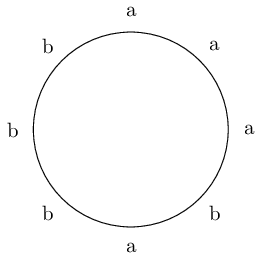
\includegraphics[scale=0.4]{circle.png}
\end{center}

Við getum skoðað hlutstrengi af lengd $n$ inni í þessum hringstreng. Tveir
hlutstrengir af lengd $3$ eru \texttt{aaa} og \texttt{aab}, eins og sjá má á
eftirfarandi myndum:

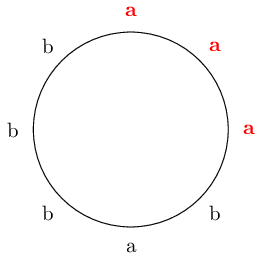
\includegraphics[scale=0.4]{circle_2.png}
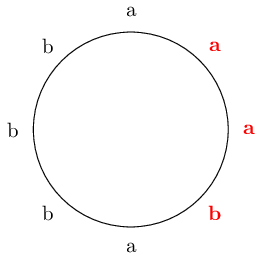
\includegraphics[scale=0.4]{circle_3.png}

Ef svona er gengið um hringinn, þá fáum við eftirfarandi $8$ hlutstrengi af
lengd $3$:
\begin{itemize}
    \item aaa
    \item aab
    \item aba
    \item bab
    \item abb
    \item bbb
    \item bba
    \item baa
\end{itemize}

Takið eftir að engir tveir þeirra eru eins.

Strengur $s$ af lengd $k^n$ sem inniheldur bara fyrstu $k$ ensku lágstafina er
kallaður $k,n$-De Bruijn strengur ef allir hlutstrengir í hring-útgáfunni af
strengnum af lengd $n$ eru mismunandi. Við sjáum því að strengurinn
\texttt{aaababbb} er $2,3$-De Bruijn strengur.

\section*{Inntak}
Inntak inniheldur tvær línur. Fyrri línan inniheldur tvær heiltölur $k$ og $n$,
þar sem $2 \leq k \leq 26$, $1 \leq n \leq 20$ og $1 \leq k^n \leq 5 \cdot
10^5$. Seinni línar inniheldur streng $s$ af lengd $k^n$ sem inniheldur bara
fyrstu $k$ ensku lágstafina.

\section*{Úttak}
Ein lína sem inniheldur \texttt{De Bruijn} ef $s$ er $k,n$-De Bruijn strengur,
eða \texttt{Neibb} annars.

